\documentclass{article}

\usepackage[utf8]{inputenc}
\usepackage{amsmath}
\usepackage{indentfirst}
\usepackage{verbatim}
\usepackage{cite}
\usepackage{graphicx}
\usepackage{array}
\setlength{\extrarowheight}{.5ex}
\usepackage{amssymb}
\usepackage{graphicx}
\usepackage{algorithm}
\usepackage{algpseudocode}

\graphicspath{./}
\usepackage[margin=1in]{geometry}

\makeatletter
\newcommand*{\shifttext}[2]{%
  \settowidth{\@tempdima}{#2}%
  \makebox[\@tempdima]{\hspace*{#1}#2}%
}
\newcommand{\hella}{\bBigg@{4}}
\newcommand{\hellla}{\bBigg@{5}}
\newcommand{\indicate}{\text{I} \shifttext{-3pt}{I}}
\newcommand{\msp}{\text{ }}
\makeatother

\title{Deep Learning Final Project: Binary Neural Networks}
\author{Brandon Duderstadt}

\begin{document}
  \maketitle
  \section{Motivation and Problem Statement}

    Deep neural networks are currently the top performing algorithm on a wide range of artificial intelligence tasks, ranging from object recognition, to complex system control, to natural language processing.
    Many of these tasks are critical components of real time robotic systems, and thus, deep neural networks have become increasingly popular in the robotics community.
    However, these networks come with a major drawback; their computational cost at inference time is prohibitively high.
    This renders the networks very slow on many embedded robotics applications, and unfit for use in scenarios requiring low resource, real time computation.\\[6pt]

    The main computation taking place in these networks is the multiply-accumulate operation, as each artificial neuron essentially computes a weighted sum of its inputs.
    Naturally, a reduction in the time cost of this operation would result in a huge savings in total network inference complexity.
    In particular, if the weights of each artificial neuron were constrained to either -1 or 1, the 32-bit floating point multiply-accumulate operations taking place at each neuron could be replaced with a much faster 1-bit XNOR-count operation.\\[6pt]

    Unfortunately, the optimization problem associated with solving for these weights is a 0-1 integer program, which is NP-Complete.
    This renders direct optimization methods ineffective. Furthermore, traditional nonconvex optimization methods, such as gradient descent, are difficult to apply here, since the XNOR operation does not have a continuous derivative.
    The resulting question is thus: \\[6pt]
    \textbf{How can one train a binary neural netowrk such that they can take advantage of the speed increase related with using XNOR-accumulate operations as opposed to multiply-accumulate operations at inference time?}

  \section{Prior Work}
    Courbariaux et. al (2016) \cite{bnn} present the current state of the art algorithm for learning these weights through a series of train-time approximations and weight-clipping. I will use this algorithm as a basis for my investigations.

  \section{Datasets}
    For my investigations, I will be using the MNIST \cite{mnist} dataset. I have selcted this dataset since it is a canonical benchmark dataset in the machine learning world.

  \section{Methods}
    The primary module that I will be using in my investigations will be a \textbf{Binary Linear Unit} (BLU). The algortihm below defines the behavior of this unit during the forward pass:\\[6pt]

    \begin{algorithm}
      \caption{Binary Linear Unit Forward Pass}\label{BLUfp}
      \begin{algorithmic}
        \Require{$X$ is the input tensor}
        \Require{$W$ is the non-binary layer weight matrix}
        \Require{$B$ is the non-binary layer bias matrix}
        \\
        \Function{Forward}{$X$, $W$, $B$}
          \State $W_b \leftarrow \text{Sign}(W)$
          \State $B_b \leftarrow \text{Sign}(B)$
          \State $X \leftarrow xW_b + B_b$
          \State $X \leftarrow \text{Sign}(X)$
          \State \Return $X$
        \EndFunction
      \end{algorithmic}
    \end{algorithm}

    The main idea to note here is that, during training time, the network stores its weights as 32-bit floats.
    However, during the forward pass, the network uses \textbf{only the signs} of the weights.
    In this way, the inference step of the BLU requires only binary weights.\\[6pt]

    One drawback of the above function is that it makes heavy use of the sign operation, which has derivative 0 almost everywhere.
    Thus, the backward pass of the BLU ignores the presence of the sign function, and passes the gradient straight through to the next operation in the operation tree.
    While this does not approximate the true gradient of the function, it allows the signal from backpropegation to continue through the network without dying out at the sign operations.\\[6pt]

    The authors of the paper suggest a series of additional network tweaks to promote training stability. The three main methods suggested by the authors are:
    \begin{enumerate}
      \item Clipping the network weights to $[-1, +1]$ after every iteration
      \item The inclusion of dropout layers between BLU's
      \item Clipping the network gradients to $[-1, +1]$ at every BLU
    \end{enumerate}


  \section{Experiments}
    For my experiments, I utilized the architecture suggested by Courbariaux et. al \cite{bnn} in the binary neural network paper.
    In particular, this is a fully connected network with 3 hidden layers of 2048 layers each.
    The authors of the paper utilize a support vector machine as the final layer of their network, but I replace this with a softmax classifier for simplicity.
    All networks were trained using the same random seed, and with the default settings of the Adam optimizer, as specified in the paper.
    Table \ref{table:testmatrix} reports the peak validation accuracy of this architecture when trained over 15 epochs, with the specified network tweaks.\\[6pt]

    \begin{table}
      \centering
        \begin{tabular}{|l|l|l|r|}
          \hline
          Weight Clipping & Dropout & Gradient Clipping & Peak Validation Accuracy\\
          \hline
          \hline
          & & & 78\% \\
          \hline
          \checkmark & & & 78\% \\
          \hline
          & \checkmark & & 44\% \\
          \hline
          & & \checkmark & 78\% \\
          \hline
          \checkmark & \checkmark & & 43\%\\
          \hline
          \checkmark &  & \checkmark & 78\%\\
          \hline
          & \checkmark & \checkmark & 42\%\\
          \hline
          \checkmark & \checkmark & \checkmark & 43\%\\
          \hline
        \end{tabular}
        \caption{Test Matrix}\label{table:testmatrix}
    \end{table}

    A few interesting observations can be made from Table \ref{table:testmatrix}.
    First, the inclusion of dropout layers in the network seem to make the network perform strictly worse in terms of peak validation accuracy.
    One potential explanation for this is that the dropout layers are eroding away too much of the signal in the forward pass, and thus, the network is having difficulty learning at all.
    One potential solution to this would be to reduce the probability of dropout at each layer as a way to promote a stronger signal in the forward pass.\\[6pt]

    The second interesting tendency in the table is that the peak validation accuracy does not seem to respond to either weight or gradient clipping.
    While this may suggest that weight and gradient clipping do not have an effect on the network performance, the validation accuracy versus iteration curves of Figure \ref{figure:overfit} tell a different story.

    \begin{figure}[h!]
      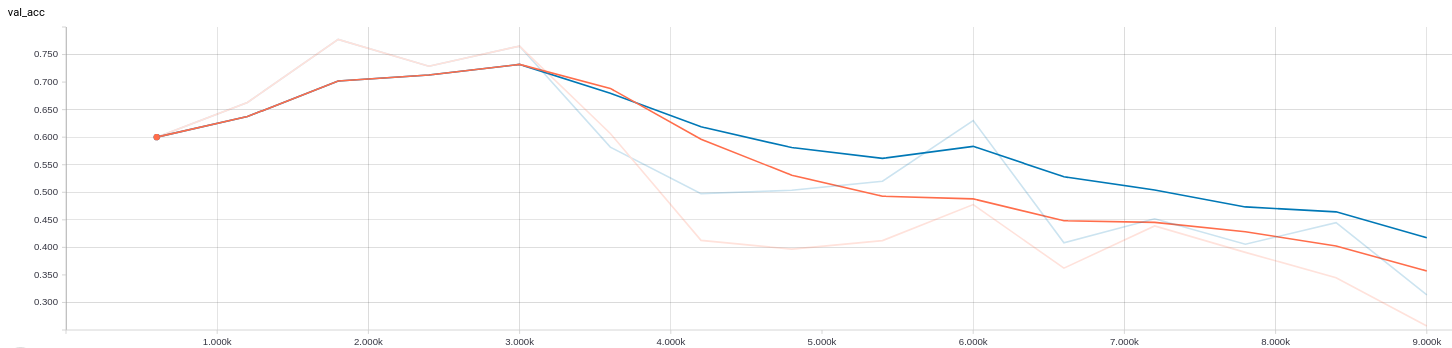
\includegraphics[scale=.33]{img1.png}
      \caption{Baseline Network (Orange) and Weight Clipped Network (Blue) Validation Accuracy vs Iteration} \label{figure:overfit}
    \end{figure}

    Figure \ref{figure:overfit} deomonstrates that clipping the weights of the network dramatically reduces the rate at which the network overfits.
    However, no such trend is present in the gradiet clipping curve.
    From this, it seems that the best strategy for the problem at hand, with respect to the tweaks suggested in the paper, is to only clip the weights of the network.
    With this being said, it is still clear that the network is dramatically overfitting.\\[6pt]

    A this point, I diverge from the paper in an attempt to get the network accuracy as high as I can.
    It is clear that the network needs to be further regularized, as it is overfitting.
    However, traditional regularization based on the magnitude of the weights does not apply here, since the weight values are already restricted to $\pm 1$.
    Furthermore, the above experiments show that dropout (with probability .5) degrades the signal in the forward pass too much to be useful as a regularizer.
    For these reasons, the following changes were made to the network:
    \begin{enumerate}
      \item The batch size was increased in order to promote more accurate gradient measurements at each iteration. This will help prevent the network from overfitting to batch effects in the data.
      \item Training data augmentation was employed to further regularize the network by preventing overfitting across epochs. Specifically, small random rotations, small random crops, and small random color jitters were applied to the input.
    \end{enumerate}

    \begin{figure}[h!]
      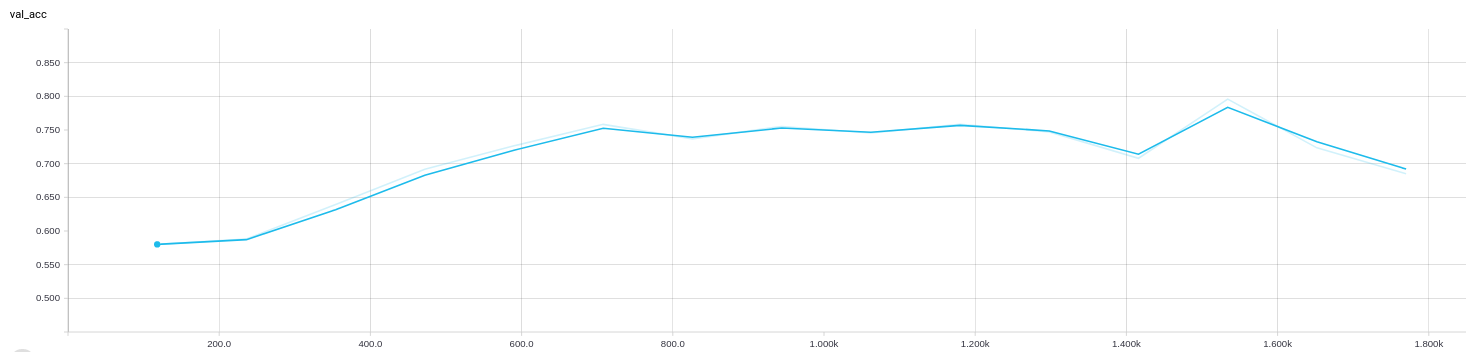
\includegraphics[scale=.33]{img2.png}
      \caption{Validation Accuracy vs Iteration in the Regularized Network} \label{figure:fix}
    \end{figure}

    Figure \ref{figure:fix} shows that these regularization measures have stabalized the training into the later epochs.
    Note that the decline in validation accuracy with increasing iteration present in Figure \ref{figure:overfit} is not present in \ref{figure:fix}.
    Furthermore, the regularized network achieves a new peak validation accuracy of $80\%$.\\[6pt]

    One final experiment was carried out in order to push the accuracy of the network as high as it could go.
    In this experiment, the width of each of the hidden layers in the network was increased to $4096$.
    The validation accuracy vs iteration curve of the larger regularized network is show in Figure \ref{figure:best}.
    This figure achieves the highest peark validation accuracy of all networks studied at $85\%$.

    \begin{figure}[h!]
      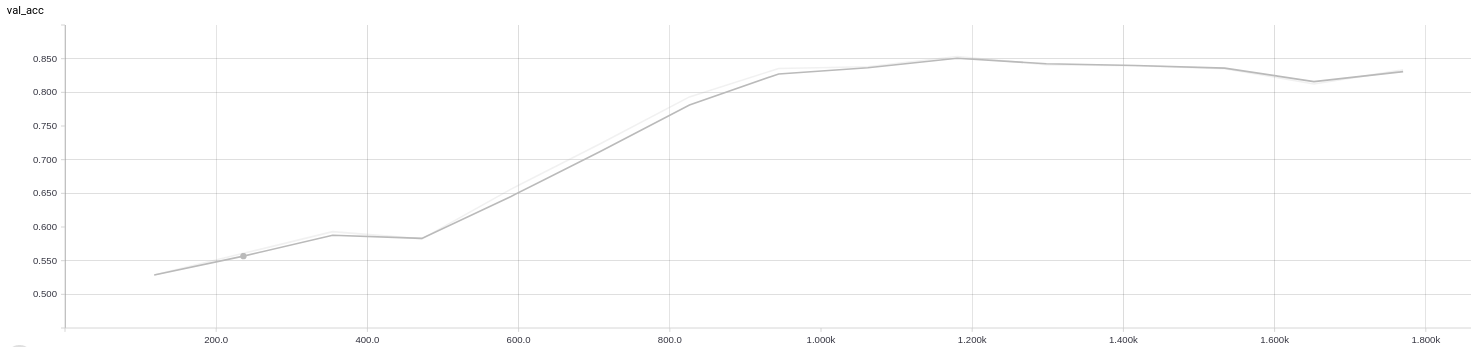
\includegraphics[scale=.33]{img3.png}
      \caption{Validation Accuracy vs Iteration in the Larger Regularized Network} \label{figure:best}
    \end{figure}


    \section*{Conclusion and Future Work}
      In this report, I have presented an overview of Courbariaux et. al's (2016) \cite{bnn} method of training binary neural networks.
      I have implemented thier method as the Binary Linear Unit (BLU) class in pytorch, and used this implementation to test a series of suggested network tweaks.
      I have deomonstrated that, in low epoch scenarios, the only of the suggested network tweaks that seems to be useful is clipping the weights to the interval $[-1, 1]$.
      Furthermore, I have shown that the overfitting issues associated with the network can be alleviated by way of training data augmentation and increased batch size.
      Finally, I have created a neural network, with purly binary weights, that can achieve $85\%$ validation accuracy on the MNIST dataset.\\[6pt]

      The analysis in this paper was constrained due to limited computational resources.
      In particular, all networks were trained for only $15$ epochs, and the only hyperparameters under consideration were those explicitly mentioned.
      Based on this, it would not be surprising to see increased performance if the networks were trained for much longer.
      Furthermore, I would not be surprised to see changes in the effects of the network tweaks if the networks were trained for, say, $1000$'s of epochs.
      In the future, I would like to redo the experiments, but with a much longer training time per network.
      Accordingly, I would like to train each network multiple times, and generate confidence intervals regarding average network performance under each of the tweaks.\\[6pt]

      All code for this project can be found at https://github.com/bstadt/binary-nn-pytorch.


  \bibliography{bib}{}
  \bibliographystyle{plain}

\end{document}
